\newpage

\section {Analyse du monde de l'édition vidéo professionnel}

\paragraph{}
Le montage vidéo professionnel est un domaine très vaste, et l'on peut
s'attendre à ce que les besoins auxquels doivent répondre les logiciels
permettant de produire les différents types d'œuvres audiovisuelles
varient fortement en fonction du type de contenu. Afin d'étudier
les possibilités d'avenir des logiciels libres dans ce domaine, il nous faut
définir, pour en connaître les différents besoins:
\begin {itemize}
  \item {les cas d'utilisation (plus communément appelées use-cases) FIXME -> index}
  \item {les fonctionnalités qui en découlent}
\end{itemize}


\paragraph{}
Nous allons donc définir les principaux cas d'utilisation en fonction des
différents types de productions audiovisuelles et ainsi en déduire les fonctionnalités
nécessaires pour répondre à ces cas d'utilisation.

\paragraph{}
Ensuite on analysera la base commune des fonctionnalités nécessaires à la
production de tous ces types de production.  Pour finir
nous verrons si les besoins sont variés, et essayerons de trouver les
fonctionnalités qui sont propres à chaque type de production. Cette première
analyse a pour but de clarifier les besoins des professionnels afin de
déterminer par la suite quels sont ceux auxquels les logiciels libres répondent déjà,
ceux auxquels on peut prétendre répondre dans un futur proche, et ceux qui
sont hors du scope actuel des technologies libres.

\subsection{Les bases de l'édition vidéo}

\paragraph{}
Tout d'abord, il est évident que pour qu'un logiciel de montage puisse répondre
aux besoins de professionnels, les fonctionnalités basiques de l'édition vidéo
non linéaire doivent être couvertes, cette partie a pour but de définir quelles
sont ces fonctionnalités, et les expliquer succinctement:

\subsubsection{Définition des termes techniques}

\paragraph {}
Du fait de l'importance des termes suivant pour la compréhension de ce document,
il est nécessaire qu'ils soient défini au sein même de celui-ci.

\paragraph{Les Footages}
Les footages correspondent à toutes les sources brutes qui ont été enregistrer
et a partir desquels, le monteur va créer le rendu final de l'œuvre 
audiovisuel.

\paragraph{Les clips}
Les clips correspondent dans les faites à un footage éditer (retouche des
couleur, modification de la durée, ajout d'effets\ldots) par le monteur
afin de l'utiliser dans un context précis de l'œuvre finale.

\subparagraph{Les templates}
Dans l'édition video, on parle de template pour définir un moule de montage.
Il permet au monteur de par la suite monter très rapidement des oeuvres en
s'assurant que le rendu rentre dans un cadre définit précédemment.

\paragraph{Colorimétrie (retouche des couleurs)}
En édition vidéo la colorimétrie est l'art de retoucher les couleurs,
les étalonner au travers des différents clips.

\begin{wrapfigure}{r}{0.5\textwidth}
   \vspace{-20pt}
    \begin{center}
      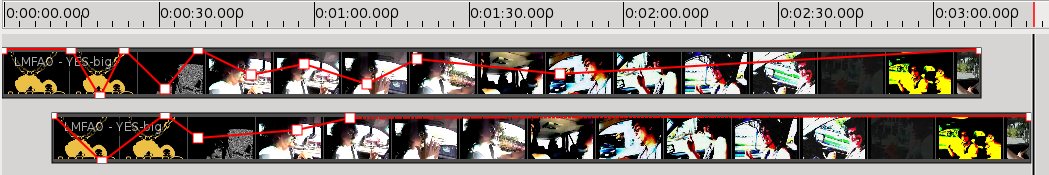
\includegraphics[width=0.48\textwidth]{images/keyframecurves}
    \end{center}
   \vspace{-30pt}
   \caption{Les keyframes}
   \vspace{-10pt}
   \label{Yes}
\end{wrapfigure}
\paragraph{Les keyframes}
Les keyframes définissent le de point de départ et de fin d'une animation,
en particulier dans le cadre d'effet, de text en mouvement au dessus
d'une vidéo\ldots

\paragraph{Speed control et time remmaping}
Le speed control permet de modifier la vitesse de lecture d'un clip dans la
timeline (ralentir où accélérer). Le time remapping est une technique avancé
de speed control, et permet de changer la vitesse de lecture de partie de clip,
et ainsi accélérer ou ralentir des partie d'un même clip. Cette technique est
couplé au keyframes afin d'obtenir le résultat souhaité.

\paragraph{Gestion des Footages}
Un logiciel d'édition vidéo doit permettre d'importer les Footages à partir %FIXME index
desquels on veut faire le montage, c'est à dire les fichiers vidéos, audios,
et images avec lesquels on travaille. Il doit être possible de prévisualiser ces
clips.

\subsubsection{Definition du concept d'édition timeline}
\paragraph{}
La timeline, est la partie de l'interface dans laquelle on va disposer les
différents clips. Il s'agit du concept de base de l'édition vidéo non-linéaire.
Dans le cadre de l'édition timeline, quelques fonction sont absoluments
indispensable, et il est nécessaire de comprendre ces différents concepts
pour comprendre la suite de ce document:

\paragraph{Découpages des clips}
  \begin{wrapfigure}{r}{0.6\textwidth}
    \vspace{-20pt}
    \begin{center}
      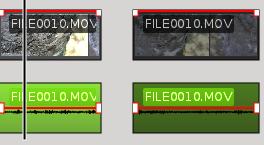
\includegraphics[width=0.38\textwidth]{images/splited}
    \end{center}
    \vspace{-20pt}
    \caption{Spliting}
    \label{No}
  \end{wrapfigure}
La technique du decoupage de clip permet de diviser un footage en plusieurs
partie afin de pouvoir les utiliser de manière indépendante.

\paragraph{}
\paragraph{Unlinking de la piste audio et de la piste vidéo}
  \begin{wrapfigure}{r}{0.6\textwidth}
    \vspace{-20pt}
    \begin{center}
      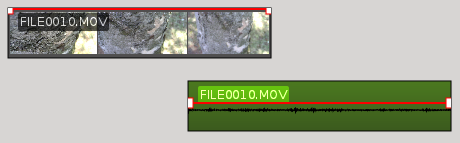
\includegraphics[width=0.38\textwidth]{images/unlinked}
    \end{center}
    \vspace{-20pt}
    \caption{Unlinking}
    \label{Yes}
  \end{wrapfigure}
Le fait de ``des lier'' les clip permet de gérer de manière desynchroniser le son
et la video.

\paragraph{Gestion des in point et  out point des clips} %Should that be translated?
  Permet de définir le partie d'un footage à utilisé dans le montage final. Cela permet donc de
  redéfinir la longueur d'un clip dans la timeline, en ne jouant pas le debut
  ou la fin de celui-ci.

\paragraph{}
\paragraph{Notion de layer}
  \begin{wrapfigure}{r}{0.6\textwidth}
    \begin{center}
      \vspace{-20pt}
      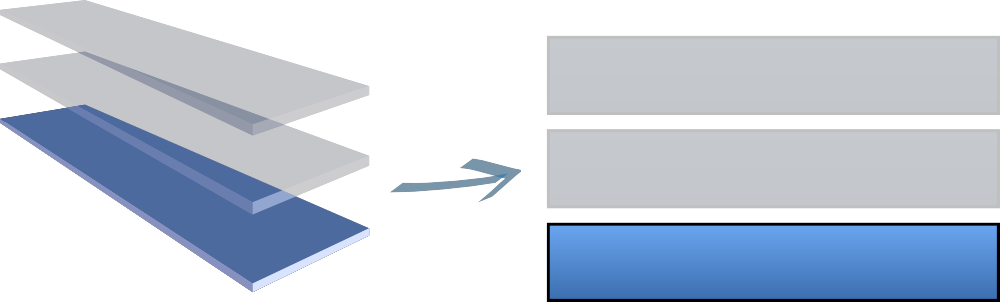
\includegraphics[width=0.38\textwidth]{images/layers}
    \end{center}
    \vspace{-20pt}
    \caption{Les layer}
    \label{Yes}
  \end{wrapfigure}
La notion de layer est essentielle dans l'édition video avancé dans la
timeline, mixer plusieurs sources et ajouter des titres depend de cette
fonctionnalité. Afin de comprendre, il est plus simple de faire la comparaison
avec de la peinture sur verre. Avec plusieurs vitres superpose les unes au
dessus des autres, chacune de ces vitre représentant un layer. Si vous
dessiner seulement sur une partie des vitre de la couche supérieur, les vitres
inférieurs vont être visibles, et ce qui sera dessine dessus sera donc visible.
De plus, il existe un notion d'opacité dans les layer, et dependant de celle-ci,
les layers inférieurs, ou non.

\subsection{Définition du marché par segment}
\paragraph{}
Dans un premier temps, nous allons définir et analyser les
différents formats de productions audiovisuelles professionnelles.
Nous avons interviewé
différents monteurs professionnels, afin de définir leurs besoins,
(annexes 1) en essayant de
couvrir le maximum de champs de l'édition vidéo. Nous
avons pu récolter des informations provenant de monteurs de clips
vidéos, de courts métrage, de publicités et de reportages.

\paragraph{}
La littérature dans la matière (En particulier \cite{WorldVideoNonlinearEditingMarket})
nous propose de faire une nette distinction entre  les deux segments du marché que sont:
\begin{itemize}
  \item {le monde du contenu post-produit: il s'agit de contenu dont la qualité de
    montage final est très importante. Celui-ci peut être de courte durée, tels que les clips
    vidéos ou publicités, où de longue durée, tels que les films, où séries télévisées. Mais
    il faut toutefois faire une différence entre ces derniers puisque la qualité du
    rendu final des films implique d'autres standards en terme de montage}
  \item {le monde de la production diffusée: il s'agit du contenu retransmis à la fois,
    sur internet, et sur les chaînes de télévisions et dont la création et la retransmission
    rapide impliquent des moyens spéciaux afin de permettre de créer et retransmettre
    le contenu dans un temps restreint, voir en direct.}
\end{itemize}

\paragraph{}
Certes les deux mondes ont des contenus différents, mais surtout ils ont des contraintes différentes,
ce qui implique des divergences importantes en terme de besoin de fonctionnalités. Nous allons donc
nous intéresser à ces deux domaines et découper notre analyse à partir de cette distinction. Tout
d'abord, nous nous intéresserons aux fonctionnalités logicielles nécessaires à la production
de contenu post-produit, par la suite, nous analyserons les besoins intrinsèques à la production de contenu
visant le monde de la vidéo diffusée. Puis nous essayerons de voir où se situe la frontière entre ces
deux mondes afin de pouvoir par la suite nous rendre compte de ce que l'investissement de ces marchés
implique pour les logiciels de montage vidéo libres.

\paragraph{Le monde du contenu post-produit}
\subparagraph{}
Le monde du contenu post produit est assez vaste, au première abord il peut apparaître comme étant tout le contenu
qui n'est pas diffusé instantanément. Dans les faits, la distinction est plus complexe, et il s'agit
d'œuvres audiovisuelles dont le temps de post production n'est pas un critère de première d'importance
pour le choix des moyens mis en place à ce sujet.

\subparagraph{}
De ce fait, les formats suivants peuvent être considérés comme étants post produits:

\paragraph{Les courts métrages}

\subparagraph{}
Les courts métrages concentrent en moins de 35 minutes, une histoire. Ils sont donc soumis
à des contraintes importantes.Puisqu'ils répondent à cette exigence de concision,
il est intéressant de se poser la question de savoir si dans ce genre
d'œuvre, les monteurs utilisent des techniques qui permettent
de les rendre plus dynamiques et si des fonctionnalités spéciales sont utilisées dans
ce but.

\subparagraph{}
Dans la production de ce type d'œuvre, les interviews, nous ont permis de mettre en évidence
les fonctionnalités qui sont indispensables telles que:
\begin{itemize}
  \item{Transition (fading en priorité)}
  \item{Effets basiques tels que le passage en noir et blanc\ldots}
  \item{Time remmaping}
  \item{Retouche des couleurs}
  \item{Création et ajout de génériques}
\end{itemize}

\paragraph {Les publicités}
\subparagraph{}
La publicité peut s'apparenter au court métrage puisqu'il s'agit de création
courte et généralement dynamique mais dont la visée est différente. Pour atteindre
leur objectif (attirer des consommateurs), les monteurs utilisent des
techniques spéciales mais les fonctionnalités du logiciel nécessaires restent
identiques.

\subparagraph{}
En revanche, la qualité du rendu est très importante, aussi des logiciels spécialisés
sont fréquemment utilisés afin de créer le contenu (audio, effets, images\ldots).

\paragraph {Les clips vidéos}
\subparagraph{}
Le clip vidéo est un contenu visuel qui a pour but d'illustrer
une musique. Ce type de vidéos utilise souvent beaucoup d'effets spéciaux, et demande à
priori une très grande précision au niveau de la synchronisation
entre le son et l'image. La track audio dans de telle production
sera de préférence effectuée avec un logiciel dédié à cet
effet. Pour résumer, les fonctionnalités nécessaires sont:
\begin{itemize}
  \item{Création de titres complexes (Titre en mouvement, etc\ldots)}
  \item{Ajout de titres}
  \item{Ajout d'effets}
  \item{Utilisation avancé des keyframes}
  \item{Time remapping}
\end{itemize}

\paragraph {Les films}
\subparagraph{}
La production cinématographique bénéficie de budgets beaucoup plus élevés, les techniques,
employés dans le cadre de la post production sont plus complexes et permettent de soigneusement
gérer la qualité du rendu.

\subparagraph{}
Il n'a pas été possible d'interviewer de monteur de film jusqu'à maintenant, mais
le livre ``The technique of film and video editing, History, Theory, and Practice''
\cite{TheTechniqueOfFilmAndVideoEditing} est un bon point de départ pour
comprendre le montage cinématographique et la très grande influence qu'il a
sur les autres type de productions audiovisuelles. On peut considérer le film comme
étant l'œuvre audiovisuelle par excellence. %FIXME formulation pourri

\subparagraph{}
Dans le monde du cinéma, le logiciel de montage vidéo est l'un des logiciels
parmi un système connecté de logiciel de post production. Des spécialistes de
différents domaines créent les parties du film, et le monteur a pour mission
de lier tout ces éléments au travers du logiciel de montage. Les logiciels
de post production sont entre autres:
\begin{itemize}
  \item{Éditeur de son}
  \item{Création d'effet}
  \item{Retouche d'image}
  \item{Création d'animation}
  \item{\ldots}
\end{itemize}

\subparagraph{}
Les logiciels à visée professionnel ne sont donc pas forcément utilisables dans
le monde de la création cinématographique. Il conviendra de faire une réelle
différence entre ces deux univers du montage vidéo.

\subparagraph{}
Ce qui résulte dans le fait que le logiciel de montage vidéo à proprement parler ne
demande pas vraiment de fonctionnalités très évoluées, la base de l'édition
et la possibilité d'organiser l'immense quantité de Footages de manière efficace
semblent être les seuls éléments clefs dans ce domaine. Les autres logiciels de
post production sont bien évidemment aussi nécessaires afin de permettre de faire
le montage de films, mais cela est un élément auquel ce document n'est pas destiné
à répondre dans le détail.

\subparagraph{}
Une autre caractéristique de la production cinématographique, qui découle une
fois de plus du fait que la qualité du résultat doit être irréprochable, est
que les logiciels de montage doivent permettre de visualiser chaque image du
film de manière très précise (le montage de film se fait dans certain cas en
choisissant chaque image depuis un tableau de frames). INDEX

%FIXME, faudrait plus détailler ici?

\subparagraph{}
Bien que ne demandant pas vraiment de fonctionnalités très avancées, la création
de film a des besoins assez évoluées en ce qui concerne le logiciel de montage:
\begin{itemize}
  \item{Organisation très avancée des Footages}
  \item{Création et ajout de générique}
  \item{Passerelles avec le reste des logiciels de post production}
  \item{Preview de chaque frame dans le détail}
\end{itemize}

%TODO essayer de trouver des monteurs de films!

\paragraph {Les séries télévisées}

\paragraph{}
Le niveau de qualité des séries télévisées n'étant pas aussi élevé que pour
le montage des films, les traitements sont la plupart du temps réalisés
directement dans le logiciel de montage même. Cela implique un nombre de
fonctionnalités plus important avec comme nécessité:
\begin{itemize}
  \item{Création et ajout de titre}
  \item{Création et ajout de générique}
  \item{Retouche des couleurs}
\end{itemize}

\paragraph {Les documentaires}
\paragraph{}
Le documentaire est en général assez sobre en terme de montage, il est en
fait, pour la plupart, dans le logiciel de montage, mais ne demande pas
de fonctionnalités spéciales. En général, les fonctionnalités utilisés
pour produire ce type d'œuvre sont:
\begin{itemize}
  \item{Création et ajout de titre}
  \item{Création et ajout de génériques}
  \item{Retouche des couleurs}
  \item{Utilisation des keyframes}
  \item{Transition smpte\footnote{smpte: Society of Motion Picture
    and Television Engineers, est une association internationale,
    située aux É.-U., et composée d'ingénieurs. Elle développe
    des standards vidéos (elle en a déjà plus de 400 à son actif),
    qui sont utilisés par exemple par la télévision, ou le cinéma numérique
    (Source: http://fr.wikipedia.org/)}}
\end{itemize}

\paragraph{Le monde du contenu diffusé}

\paragraph{}
La plupart du contenu post produit est par la suite diffusé, la différence que l'on
fait ici entre ces deux types de production réside dans le temps de la post production.
Dans le cas des journaux télévisés, émission de télé, la post production est soit totalement
inexistante (dans le cas du direct), soit très courte, dans le cadre de reportages, jeux télévisés
et autres types de production visant spécifiquement la télévision.

\paragraph {Les émissions télévisées}
\paragraph{}
Les émissions de télévision peuvent selon la manière dont elles sont produites être
classées plutôt dans le contenu post-produit, où dans le contenu diffusé, mais par le
fait qu'elles sont en général diffusées très rapidement après la création du contenu (si ce n'est en
direct), il convient de les considérer comme du contenu diffusé. De plus le fait qu'elles soient
produites exclusivement pour la diffusion (aucune commercialisation matérielle n'en est faite), cette
classification paraît naturel.

Du fait de leur temps de production très réduit, les principales fonctionnalités en terme de logiciel
de montage sont:
\begin{itemize}
  \item{Fonctionnalité de template qui permet d'avoir un cadre général de montage de
    présentations, au moment voulu et ainsi faire le montage en direct}
  \item{Titres}
\end{itemize}

\paragraph{}
Bien évidemment, dans le cadre de la création de template, les transition ``smpte'' et les effets simples
sont généralement utilisés. Mais il n'est pas rare que les template à proprement parler ne soient pas créés
dans le logiciel de montage, mais plutôt dans d'autres logiciels de création de contenu audiovisuel.

\paragraph {Évènements spéciaux (sportif, d'actualité\ldots)}

\paragraph{}
Ce type de production audiovisuelle n'est en principe absolument pas post-produit. Il
s'agit de production instantanée, et pour ce type de contenu, l'outil de montage non
linéaire doit permettre de donner une impression de contenu post-produit alors
qu'il n'en est rien. Les fonctionnalités nécessaires sont assez similaires
à celles dont on aurait besoin pour produire des émissions de télévision.

\subparagraph{}
De plus, l'acquisition étant aussi fait en direct, il doit être possible
d'intégrer le logiciel du montage dans le système de capture d'image et de son.

De même que pour les émissions de télé, les template sont généralement produits avec des logiciels
dédiés à cet effet.

\subsubsection{Analyse des fonctionnalités communes}

\paragraph{}
On s'aperçoit donc que de nombreuses fonctionnalités sont communes aux différents
types d'œuvres. Il convient de détailler chacune de ces fonctionnalités afin de
nous rendre compte de ce qu'elles impliquent en terme de logiciel de montage.

\paragraph{Création et ajout de titre}
\paragraph{}
Cette fonctionnalité est utilisée dans la création de plusieurs types de contenu:
\begin{itemize}
  \item {Séries télévisés}
  \item {Documentaires}
  \item {Clips vidéos}
\end{itemize}

\paragraph{}
Bien que cette fonctionnalité soit utilisée dans ces différents types de contenu,
ce qu'elle implique dans le logiciel à proprement parler peut varier en fonction
de différents paramètres. Par exemple, dans une série télévisée en général le
travail sur les titre sera assez limité, on aura en général une vidéo en arrière-plan
et un titre que fera un fondu arrière. Alors que dans le cadre de clips vidéo,
il sera fréquent que le titre soit en mouvement et qu'il suive le rythme de la
musique par exemple. Afin de répondre au besoin du plus grand nombre, il faudrait
pouvoir répondre à ces différent cas d'utilisation, mais il sera plus difficile
aussi bien en terme de backend qu'en terme d'interface utilisateur de répondre
aux besoins le plus spécifiques.

\paragraph{Création et ajout de générique}
\paragraph{}
La création de générique est une fonctionnalité indispensable, à laquelle de
nombreux monteurs (en particulier professionnels) font appelle. Cette
fonctionnalité en terme de backend est similaire à
celle des titres puisqu'il s'agit ni plus ni moins d'ajouter du
texte au dessus d'un fond qu'il soit animé ou non. Mais en terme d'UI
\footnote{UI: User Interface, il s'agit du terme  très largement
employé pour définir l'interface utilisateur, en général graphique (GUI)},
il s'agit de deux fonctionnalités différentes puisque par définition,
le générique est un texte qui défile dans une très grande majorité
des cas, de haut en bas.

\paragraph{}
Cette fonctionnalité est l'une des plus basiques si
l'on veut pouvoir répondre aux besoins des professionnels. Elle est utilisée
dans la plupart des créations vidéo et doit être à priori standardisée et
simple à utiliser dans l'interface utilisateur afin que la mise en place
des génériques (déjà écrits) soit effectuée de manière simple et rapide
par les monteurs.

\paragraph{Gestion des Keyframes:}
\paragraph{}

Les keyframes sont utilisées dans bien des domaines, mais dans beaucoup de cas, elles sont
utilisées avec parcimonie. Elles permettent dans une vidéo, d'animer les propriétés
d'éléments ajoutés par le monteur (effets, texte, etc\ldots). Il
apparaît donc nécessaire d'avoir une gestion minimale des keyframes,
en particulier pour une gestion fine des couleurs, mais leur utilisation est
rarement vraiment avancée.

\paragraph{}
Dans la création de clips en particulier, afin de dynamiser la vidéo,
les monteurs utilisent de manière intensive les keyframes.

\subsubsection{Fonctionnalités spécifiques}
%Ils  que dans %FIXME
%les fait, les fonctionnalités utilisés sont assez similaire bien que
%les œuvres finales soient totalement différentes.

\paragraph{}
Quelques fonctionnalités sont apparues comme vraiment propres à la création
d'un type d'oeuvre en particulier.

\paragraph{Visualisation image par image:}
\begin{wrapfigure}{r}{0.5\textwidth}
    \begin{center}
      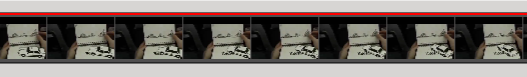
\includegraphics[width=0.48\textwidth]{images/frameByFrame}
    \end{center} \caption{Visualisation frame par frame} \label{Yes}
\end{wrapfigure}

Dans le cadre de la création de film, la prévisualisation de chaque frame,
de manière précise semble être une fonctionnalité essentielle,
cela signifie, que le logiciel de montage doit permettre de
voir de manière simple chaque frame des vidéos présentes dans la
timeline. Cette fonctionnalité est aussi utile dans le cadre de
la création d'autres oeuvre, mais est indispensable dans le cadre
de film, afin de s'assurer de la qualité du résultat. En effet,
lors de la création d'un film, chaque frame doit être contrôlée,
alors que dans d'autres types d'oeuvre, les exigences étant moins
élevées ainsi que les moyens, une telle fonctionnalité ne est pas
indispensable.

\paragraph{Gestion avancée des Footages}
\paragraph{}
Dans le cadre de productions longues, un des problème auquel doit répondre de
manière satisfaisante le logiciel d'édition est la gestion et la classification
des Footages. Cela est en particulier vrai pour les films et les séries télévisées.
Dans ces types de production le nombre d'heures de Footages peut être très grand, et
le monteur doit dans un premier temps, établir une classification
des Footages. Le logiciel de montage doit, pour répondre aux besoins des monteurs,
permettre de les ordonner de manière précise et bien pensée.

\paragraph{Intégration dans un écosystème de logiciel de post production}

\paragraph{}
Dans le cadre de création de film en particulier, on constate qu'il est nécessaire
que le logiciel de montage puisse s'intégrer dans l'écosystème de logiciel de post
production. Cela est en général possible si ce logiciel de montage respecte les
quelques standard de la post production d'oeuvre audiovisuel comme par exemple le
Material eXchange Format \footnote{Material eXchange Format ou MXF est un conteneur
utilisé par les professionnels pour les données audio et vidéo numériques.
Il s'agit d'un format défini par des standards de la SMPTE. (Source: wikipedia)}

\paragraph{Time remapping}
\paragraph{ }
Le time remapping, comme précédemment indiqué, est particulièrement utilisé dans
la création de contenu court. Il permet d'accélérer, où ralentir une partie d'un
clip pour le rendre l'œuvre la plus dynamique possible.

\paragraph{Gestion des templates}
\paragraph{ }
La création de contenu non post produit demande des particulières. La fonctionnalité
qui apparaît comme clé pour répondre aux besoins liés à ce type de produit, est la
création de template. Par exemple, la création de journaux télévisés, ou autres évènements
sportifs (dans les faits presque tout ce qui est montage télévisé) demande une gestion avancée de ``moule``,
ou template, qui permet de simplement lier les contenus des différentes caméra
à un moment donné de la retransmission.

\paragraph{ }
Cette fonctionnalité n'est pas exclusivement utilisée dans la création de contenu en direct, mais
elle est très largement utilisée dans tout ce qui est contenu destiné à la télévision.

\paragraph{}
\paragraph{}
En conclusion, on a constaté que le champ de fonctionnalité est vaste, la plupart de ces
fonctionnalités sont génériques et leur
utilisation est commune à différents types d'œuvres. Ce qui varie particulièrement  est
la finesse d'implémentation et le niveau d'utilisation qu'en fait le monteur.

\newpage
\subsection{Comparaison des principaux logiciels présents sur le marché de
l'édition vidéo professionnel, et analyse des manques et risques du marché}

\paragraph{}
  Il conviendra d'analyse en profondeur les logiciels existants, qu'ils soient
  propriétaires ou libres. Cette partie a pour but de rendre compte de
  l'état actuel du marcher des logiciels d'édition vidéo qui ont pour principal
  public les professionnelles. Cette étude portant principalement
  sur les logiciels libres, ceux-ci seront évidemment inclus dans cette analyse
  bien que l'on puisse considérer que à cause de leur manque de maturité, ils
  n'y aient pas totalement leur place.

\paragraph{}
  Dans cette optique, on analysera les points clés des logiciels.
  Tout d'abord on comparera les fonctionnalités des
  logiciels, la manière dont elles sont gérées, et on essayera d'avoir l'avis de
  professionnels sur ces fonctionnalités et leur implémentation dans les différents
  logiciels. Ensuite on regardera le prix de ces logiciels, verra en quoi cela
  peut être un argument de poids pour les logiciels libres et leur éventuelle
  prise de part de marché. Par la suite nous nous concentrerons sur la documentation,
  livres et autres tutoriels disponibles pour ces différents logiciel, et verrons
  quels supports sont offerts aux professionnels pour ces logiciels.

\paragraph{}
  Dans cette étude, nous nous concentrerons sur les plus grands acteurs du marché que sont:
  \begin{itemize}
    \item{\textbf{Avid Media Composer:} Leader historique du marché du logiciel de montage non linéaire
      professionnel. Il s'agit du produit phare de Avid Technology publié en 1989. Depuis, ce
      logiciel a joué un rôle essentiel dans l'avènement de ce marché.}
    \item{\textbf{Avid Symphony:} Evolution de Avid Media Composer, il s'agit d'une version plus complète en terme
      de fonctionnalités qui a pour but de répondre aux besoins des monteurs de productions longues telle que
      les documentaires et les séries télévisées.}
    \item{\textbf{Final cut pro:} logiciel de montage intégré dans la suite de logiciels de post-production
          de Apple, Final Cut Studio. Il s'agit d'un logiciel de montage orienté à la fois
          professionnel et création de film. Il est de nos jours très utilisé et est devenu l'un
          des leaders mondial du marché.}
    \item{\textbf{Adobe Premiere Pro:} Logiciel de montage de la suite Adobe Creative suite, il s'agit du logiciel
      d'édition vidéo à visée professionnelle de Adobe System. Il est à la fois adapté pour la création
      de contenu diffusé, mais aussi de contenu post produit}
    \item{\textbf{Cinelerra:} Logiciel de montage libre sponsorisé par la société Héroïne. Il s'agit d'un logiciel
      de montage non linéaire avec de très nombreuses fonctionnalités. Principalement créé pour le création de contenu
      diffusé, il permet aussi de répondre aux besoins de la production de contenu post-produit.}
    \item{\textbf{Kdenlive:} Logiciel de montage libre s'intégrant dans la suite logicielle de l'interface graphique KDE.
      Ce logiciel de montage est assez complet et peut répondre aux besoins des monteurs de contenu post-produit.}
    \item{\textbf{PiTiVi:} Logiciel de montage libre encore basique mais en plein développement. Ce logiciel a pour
      but de répondre aux besoins du plus grand nombre, et en particulier à ceux des professionnels de la création de
      contenu, qu'il soit post produit où non.}
  \end{itemize}

\subsection {Historique du marché}

\subsection{Fonctionnalités}
  Tout d'abord, il convient de voir quelles fonctionnalités existent chez les différents
  acteurs du marché.
  \subsubsection{Prix}
  \subsubsection{Documentation}
  \subsubsection{Support}
